\documentclass[sigconf]{acmart}
\usepackage{booktabs} % For formal tables
\usepackage{algorithm,algpseudocode}

% Copyright
%\setcopyright{none}
%\setcopyright{acmcopyright}
%\setcopyright{acmlicensed}
\setcopyright{rightsretained}
%\setcopyright{usgov}
%\setcopyright{usgovmixed}
%\setcopyright{cagov}
%\setcopyright{cagovmixed}


% DOI
% \acmDOI{10.475/123_4}

% ISBN
% \acmISBN{123-4567-24-567/08/06}

%Conference
%\acmConference[APSys'2017]{ACM SIGOPS Asia-Pacific Workshop on Systems }{September 2-3, 2017}{Mumbai, India} 
\acmConference[]{}{}{} 
\acmYear{2017}
\copyrightyear{2017}

% \acmPrice{15.00}


\begin{document}
\title{A Performance Model for Automatic Optimization of Software Packet Processing Pipelines}

\author{Author 1, Author 2, Author 3, and Author 4}
\affiliation{\institution{Affiliation}}
\email{{author1,author2,author3,author4}@affiliation.org}

\begin{abstract}
Software packet processing is increasingly commonplace, especially
for software-defined networking constructs. Previous work has
investigated methods to efficiently map packet processing pipelines
to general-purpose processor architectures. Concurrently, novel
high-level domain-specific
languages (DSLs) for specifying modern packet processing
pipeline functionality, are emerging (e.g., P4 \cite{p4}).
An attractive goal is develop
a compiler that can automatically map a high-level
pipeline specification (specified in a high-level DSL) to an
underlying machine architecture. Ideally, the compiler should automatically
exploit the available parallelism, make intelligent scheduling decisions,
and adapt to the workload needs in an online fashion, to provide maximum
performance. An important pre-requisite for the
development of such a compiler, is a
performance model of the underlying machine architecture, for
the applications of interest.

We report our experiences with adding an optimizer
to the P4C compiler \cite{Laki:2016:HSP:2934872.2959080}, which
compiles a high-level P4 program to a lower-level C-based implementation that runs
with the DPDK infrastructure \cite{DPDK}, and gets eventually executed
on a multi-socket x86 machine. We make two contributions: (a) we show
that significant performance improvements (up to 55\%) can be gained by adding
scheduling and prefetching
optimizations to the P4C compiler; and (b) we develop a performance
model for reasoning about
the expected throughput and latency of a packet-processing workload, on a
modern machine architecture. Our model can be used by a compiler,
to reason about the expected
performance of a packet-processing workload for different code configurations, and
can thus be used to optimize the generated code accordingly.
\end{abstract}

%
% The code below should be generated by the tool at
% http://dl.acm.org/ccs.cfm
% Please copy and paste the code instead of the example below. 
%
\begin{CCSXML}
<ccs2012>
<concept>
<concept_id>10003033.10003079.10011672</concept_id>
<concept_desc>Networks~Network performance analysis</concept_desc>
<concept_significance>500</concept_significance>
</concept>
<concept>
<concept_id>10003033.10003099.10003102</concept_id>
<concept_desc>Networks~Programmable networks</concept_desc>
<concept_significance>500</concept_significance>
</concept>
<concept>
<concept_id>10003033.10003079.10011672</concept_id>
<concept_desc>Networks~Network performance analysis</concept_desc>
<concept_significance>500</concept_significance>
</concept>
</ccs2012>
\end{CCSXML}
\ccsdesc[500]{Networks~Network performance analysis}
\ccsdesc[500]{Networks~Programmable networks}
\keywords{Software Switch, Batching, Prefetching}
\maketitle
\section{Introduction}
% The rapid advancements in networking have necessitated the development of many newer protocols and packet processing functionalities. The difficulty in programming and extension of traditional hardware routers has made software routers --packet processing software running on general purpose hardware- more popular. In effect, software routers have realized the modification of network functionality with a software upgrade, avoiding the burden of hardware developers in designing and developing newer hardware.

Software defined networking is already mainstream. Newer protocols and innovative packet
processing functionalities, imply that
newer packet processing pipelines are getting developed over time. Manually
optimizing such packet processing pipelines requires highly-skilled programmers, is tedious
and time-consuming, and can be repititive.
For example, the RouteBricks paper \cite{routebricks} discusses several insightful optimizations
for a simple packet-forwarding application on a modern multi-core machine; doing such careful
research for each separate (and potentially much more complex) packet processing pipeline
seems impractical. Further, these optimizations need to be re-tuned for every different
architecture.

%The rapid advancements in networking have necessitated the development of many newer protocols and packet processing functionalities resulting the increase of length, complexity, and diversity of the code in software routers. Thus programming in low-level languages like C++ is equivalent to reinventing the wheel consuming time and effort of the programmer. The business of manual optimizations in the code further complicates the job of a programmer. For example, Routebricks achieved 24Gbps of IPv4 throughput on two quad-core Nehalem processors. But the authors had to do very careful manual tuning to achieve such performance. In spite of that, the other workloads deviating from the setup might take a significant performance hit.

Domain specific languages like P4\cite{Bosshart:2014:PPP:2656877.2656890} and Click\cite{kohler2000click}, are intended
to bridge this gap, by allowing manual specification of functionality using high-level constructs. In this way, several
low-level details are abstracted away from the programmer. However, the onus of efficiently mapping this high-level
specification to the underlying machine architecture, shifts to the compiler. The difference between an unoptimized
and optimized implementation for the same high-level specification, can be significant.
For example, Kim et. al. \cite{Kim:2012:PBC:2349896.2349910} optimize the specification of an
an IPv4 forwarding engine, specified using the Click programming model, to achieve 28 Gbps of IPv4 throughput for minimum-sized
packets
on a machine with two quad-core Intel Xeon X5550 CPUs, i.e., they achieve roughly 3.5 Gbps per CPU core for this workload.
Similarly, P4C \cite{p4c}, a prototype compiler for P4,
is able to achieve 5.17 Gbps IPv4 throughput per CPU core for an identical workload configuration, on an Intel Xeon E5-2630
CPU. In contrast, a hand optimized implementation for this workload can achieve over 10Gbps per core on an
identical machine. An ideal compiler should be able to
bridge this performance gap between compiler-generated code and hand-optimized code.

We evaluate two important compiler optimizations in this context, and evaluate their performance
effects on common packet-processing workloads running on a commodity server machine: (1) efficiently exploiting
the DMA bandwidth between NIC and main memory; and (2) efficiently exploiting the memory-level
parallelism between CPU and main memory. For the latter, we also evaluate prefetching to minimize
cache-miss stalls. Finally, we rely on existing C compilers (e.g., gcc) to automatically optimize
the generated code to efficiently utilize the CPU processor (e.g., by maximizing SIMD
and instruction-level parallelism). We experiment with several code configurations involving varying
degrees of available parallelism to DMA channels, and to CPU-memory channels. We show
improvements over previously-published performance results for similar programs, and develop a model
for reasoning about performance in this setting. We have integrated our model into the
P4C compiler, to enable it to
automatically optimize the example programs discussed in this paper.

%The key issues in software routers are due to the overheads in memory stalls and redundant operations like function calls that waste CPU cycles. On Intel x86 platforms, memory access latency is 90-130 ns. It is often the case that ineffective coding styles cause more memory accesses than necessary thus increasing CPU cycles per packet.  In addition, multiple packets during processing pass through the same function flow. Thus there is a benefit in amortizing the overheads in function calls. In this work, we leverage batching as an efficient means to hide memory stalls and amortize redundant operations. We also demonstrate forwarding performance improvements by adding batching capabilities to the P4C compiler. The primary contributions of this paper are:

%\begin{enumerate}
%\item Developed a platform agnostic mathematical relation that allows one to investigate the benefits of batching and prefetching.
%\item Extended the P4C compiler for the Intel x86 platform to generate router code. Our compiler generates batched code of the target router.
%\item Detailed performance evaluation and comparison of popular network applications like L2fwd, IPv4, IPv6, NDN with other popular manually optimized applications.
%\end{enumerate}

\section{Building Blocks}
\label{Buildingblocks}
Various components of a commodity server can be used efficiently to get the good performance for network applications. Commodity servers has mainly three components which decides the performance of the application: NIC subsystem, CPU, and Memory subsystem. In this work we are exploring batching and prefetching, and in the next subsections we will be writing about the relation of batching and prefetching with NIC, CPU, and Memory.
These subsystems can work in parallel and batching \& prefetching can be used to improve the application performance.

CPU can perform out of the order execution when memory subsystem is busy fetching the data. We can exploit this fact to make CPU and memory subsystem work in parallel. Prefetching works more effectively when it is associated with batching. With proper batch size, we are making sure that CPU has enough work to do while memory subsystem is bringing the data into the cache. Detailed description about batching and prefetching is in section \ref{iobatching}, \ref{computationbatching}, and \ref{prefetching}.
% 
% \subsection{Intel Data Plane Development Kit}
% There are two parts of DPDK\cite{DPDK}: 1) Set of libraries, and 2) Userspace poll mode driver. DPDK drivers work in poll mode to avoid interrupt overheads and applications use the libraries to receive, process, and transmit the packets. The userspace poll mode driver and the libraries are implemented efficiently to process the packets at line rate. DPDK is using many optimizations to work at such a high speed. We are omitting the generic details about these optimizations and can be read from the official documentation. 

\subsection{Packet Processing Pipeline}
\label{overview}
There are mainly three stages in the network packet processing flow: Receive, Process, Transmit.
\begin{figure}[ht]
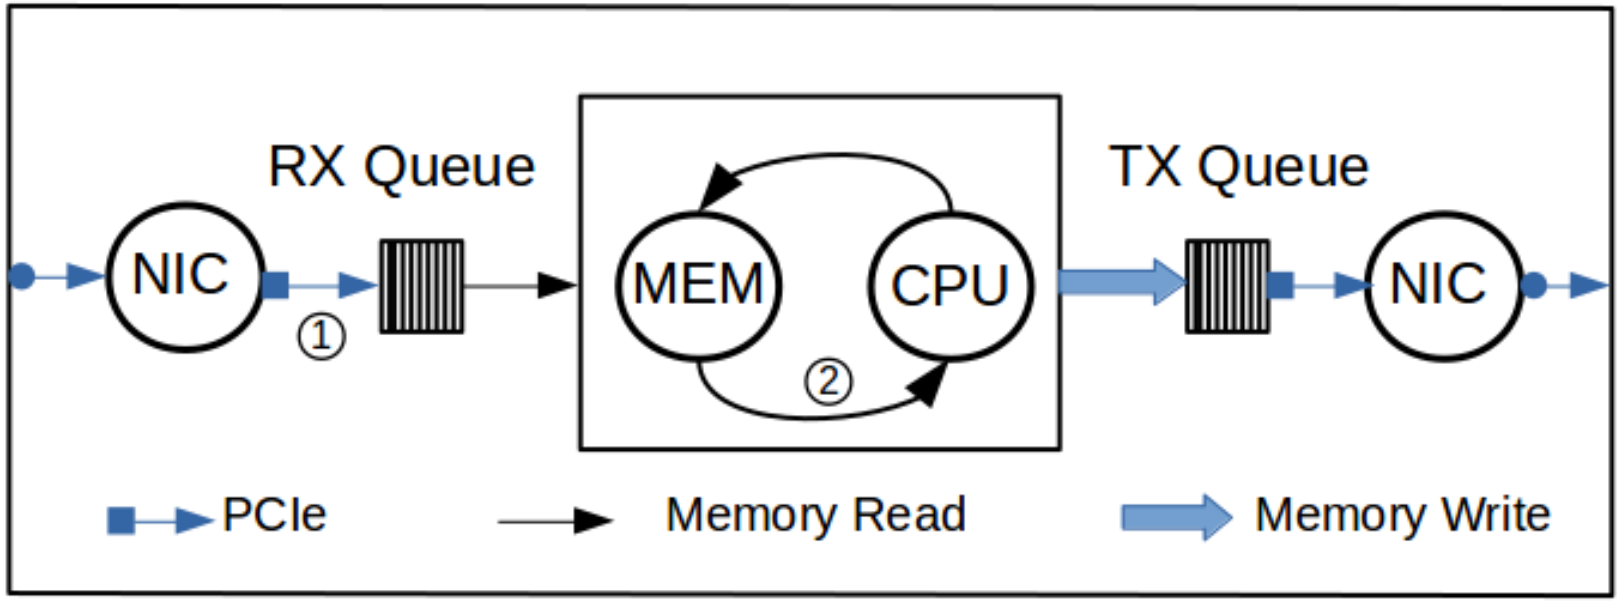
\includegraphics[width = \linewidth]{Figures/queuing.png}
\caption{Packet Processing Pipeline}
\label{overviewfigure}
\end{figure}
\\
\textbf{Receive:} After receiving data from physical layer, NIC puts the data in the buffer and then DMA engine transfers it in main memory through PCIe. Driver maintains the queue for received packets and pass the ownership to the application by reflecting it in the descriptors. When application makes a call to receive packets, poll mode driver(PMD) passes the packets to the userspace application. DPDK has library functions to RX and TX packets in batches. Descriptors are shared by NIC and PMD as a Single  Producer Single Consumer Queue and they both polls other ends of it independently.
\\
\textbf{Process:} Lookup based applications are very common in packet processing and we are more interested in such applications. The typical flow for such application involves header extraction, lookup based on header field(s), and transmission based on the lookup result.
\\
\textbf{Transmit:} This stage is very similar to receive stage in reverse direction. 

\subsection{I/O Batching}
\label{iobatching}
It can be noted in the section \ref{overview} that RX and TX of a packet is a costly process. Transferring the descriptors and packet from NIC to memory incurs overheads for each PCI transaction. For RX and TX of each packet there is a DMA overhead, PCIe overhead, and packet buffer \& descriptors management overhead. These overheads can be amortized among packets by transferring them in batches. We are using DPDK based poll mode driver which supports IO batching and has implemented the batched receive and transmit of packets in an efficient way by using vector instructions.

\subsection{Computation Batching}
\label{computationbatching}
For each packet processing there is a cost involved, an application does some sort of bookkeeping, executes many functions based on the application flow, and accesses various data structure. All this cost can be amortized among packets if we are doing all these operations in batches. In case of computation batching, all the packets pass through one stage before moving to the next stage. Instead of calling a function batch time, each function is called once and all the packets in the batch are processed together. It reduces the function call overhead. Data and instruction locality also increases because CPU executes the same portion of the code and accesses the same data structure for batch number of times before moving to next stage. Batching also allows the use of vector instructions to make packet processing more efficient.

\subsection{Prefetching}
\label{prefetching}
Software prefetching is an old concept and has been used extensively to improve the performance for memory bound applications. In Figure \ref{overviewfigure}, we are showing memory subsystem as one component, however CPU can issue multiple memory accesses and memory subsystem can fetch \#MSHRs requests in parallel. Prefetch allows the application to use memory and CPU in parallel e.g. CPU can do its work while memory system is bringing data into L1 cache. If we know that some data will be used later in the program, it can be prefetched by the prefetch instruction. In Algorithm \ref{lookup-algo} we are showing how prefetch can be used for lookup based network application. In line \ref{hash-lookup-line} we need bucket where the key is present. If we remove prefetch instruction in Line \ref{prefetch-line} CPU will stall at Line \ref{hash-lookup-line} if the bucket is not present in L1 cache. To avoid the stall we can prefetch the bucket in the first loop. This will reduce the total stall time and the performance of the application will increase.

\begin{algorithm}[H]
 \caption{HASH LOOKUP}
 \label{lookup-algo}
 \begin{algorithmic}[1]
 \For{$i \leftarrow 1$ To $Batch Size$}
     \State key-hash[i] = extract key and compute hash;\Comment{$C_K$} \label{hash-compute-line}
     \State prefetch(bucket-for-key-hash(key-hash[i]));\Comment{$C_P$} \label{prefetch-line}
 \EndFor
 \\
 \For{$j \leftarrow 1$ To $Batch Size$}
     \State value[j] = hash-lookup(key-hash[j]);\Comment{$C_L$} \label{hash-lookup-line}
 \EndFor
 \end{algorithmic}
\end{algorithm}
There is a harmony between prefetching and batching, prefetching without batching won't be very effective. It is due to batching that CPU is doing some operation on the next packet while memory subsystem is prefetching the data in parallel.

\textbf{Prefetch Distance and Batch Size:}
\label{subbatching}
Given that $C_K$, $C_P$, and $C_L$ are number of cycles needed to calculate the hash, issue the prefetch, and lookup the value respectively. We are issuing prefetch $(C_K + C_P) * (BatchSize-i) + C_L*(i-1)$ number of cycles before, where $i$ is packet number. However all the prefetches can't work in parallel and maximum \#MSHR(Miss Status Handling Registers) prefetch instructions work in parallel. So effective prefetch distance is defined by the number of free MSHRs.

Efficient use of Software prefetching is highly dependent on right prefetch distance. Prefetch distance can be explained as CPU cycles between the prefetch instruction and the instruction where data is being used. If the prefetch distance is very small then we won't be able to reduce the memory stall and there is an additional overhead of issuing prefetch instruction. If the prefetch distance is too high then the data might not be in the cache when the application needs it. For example, if the values of $C_K, C_P, and C_L$ are large and we are using large batch size then prefetch distance would be more and we might not be able to find the data when needed. In such cases we can reduce the batch size to make the prefetch distance more precise. We can form the sub batches at lookup stage instead of changing the batch size at application level.

\section{Relation between Batching and Prefetching}
\label{optimalbatchsize}
Batching has been used extensively for network applications. In our knowledge there is no model which can be used to find a relation between batching and prefetching. In this work we have tried to formulate the correlation by including important parameters, which is generic enough to be used on any platform. We need to set the optimal batch size at three levels to make the application run efficiently, IO level, CPU level, and Memory level. 

\subsection{Mathematical Model}
In this section, we are formulating the dependence between throughput and batch size. We are explaining the model form top to down to decide optimal batch size. Let
\begin{align}
B_{opt} &=  \text{arg}\,\max\limits_{(B_1, B_2)}\, (\Upsilon(B_1) , \Theta(B_2)) \label{bopt}
\\
\text{T} &= \frac{1}{\max (\Upsilon(B_1) , \Theta(B_2))} \label{overall_throughput}
\end{align}
\\
where $\Upsilon(.)$ and $\Theta(.)$ represents I/O processing and compute processing, time at given batch size for one packet, respectively. $\text{T}$ is overall processing throughput in packets per second.\\ \\
$\Upsilon(.)$ will depend on PCI bandwidth, PCI latency, NIC, DMA engine etc.
\begin{equation} 
\label{nic_throughput}
\Upsilon(B) = \Psi(\textrm{PCI, NIC, DMA engine, others})
\end{equation}
$\Theta(.)$ is directly proportional to total cycles CPUs takes to process a single packet. This includes cycles wasted by CPUs to wait for data to come from memory system. 
\\
\begin{equation} 
\label{compute_througput}
\Theta(B) \propto \Delta_{compute}(B) + \frac{\Delta_{stall}(B)}{B}
\end{equation}
Given batch size $B$, $\Delta_{compute}(B)$ represents number of cycles CPU is busy doing computation for a single packet and $\Delta_{stall}(B)$ represents number of cycles CPU  is waiting for memory operations to complete for all $B$ packets. As explained in Section \ref{prefetching}  and \ref{subbatching} CPU may stall if it needs a data which is not present in L1 cache. $\Delta_{compute}(.)$ can also vary with batch size due to increase in data and instruction locality in the memory system.
\\
$\Delta_{compute}(.)$ can be broken down into two useful terms, representing cycles which gets amortized and cycles which doesn't gets amortized due to batching.
\\
\begin{equation} 
\label{cycles_compute}
\Delta_{compute}(B) = \frac{\Delta_{shared}(B)}{B} + \Delta_{necessary}(B)
\end{equation}
Given batch size $B$, $\Delta_{necessary}(B)$ is unamortizable work that needs to be done per packet and $\Delta_{shared}(B)$ is work that is done once per batch and not per packet. For example, overheads for function calls gets amortized among the batch whereas packet header extraction needs to be done for every packet, thus, not amortizable.
\\
Average cycle stall per packet is the difference of average cycles memory system takes to bring data into caches for one packet and useful computation done on an average during that time for a packet.
\\
\begin{equation}
\label{cycles_stall}
\frac{\Delta_{stall}(B)}{B} = \Delta_{fetch}(B) - \frac{\Delta_{hide}(B)}{B}
\end{equation}
where $\Delta_{stall}(B)$ is the average latency of fetching data from memory system into caches and $\Delta_{hide}(B)$ is the work done while memory system is bringing data into caches. In Algorithm \ref{lookup-algo} CPU is doing work for another packet in batch while memory subsystem is prefetching the required data. As explained in Section \ref{prefetching}, prefetching will reduce the overall stall time. 

\textbf{Summary:} To get the maximum throughput, we need to set the optimal batch size at all the levels. Our aim is to find out the optimal batch size at IO level, CPU level and Memory level. We are assuming that packets are coming with a uniform rate. IO batch size is dependent on PCIe bandwidth and availability of on-die memory space, as far as we are using these resources efficiently we can keep the batch size minimum. At CPU, optimal batch size is dependent on the rate at which it is processing the packets and if the NIC is able to accumulate the Batch Size number of packets in that time then the batch size is optimal, until then we can increase the batch size. \textbf{Other important factor which we need to consider is the optimal use of cache, modeling }


At Memory, our goal is to minimize the stall cycles and the batch size which is giving the right prefetch distance for the prefetches would be the optimal memory level batch size. In Experiment \ref{batchvstable} we are explaining the results with the help of this model.
\section{Evaluation}
\label{evaluation}
Evaluation section is divided into four types of experiments: First, we are showing the effect of batching and batching plus prefetching for each application. Second, we are comparing our applications with the same application with hand-tuned optimizations published in different papers. By doing this we are showing that automatic optimizations can work as good as hand-tuned optimizations. Third, we are running the applications with different number of cores to show that the applications are scaling linearly with the number of cores. Fourth, we are comparing the throughput by changing the batch size and table size for L2FWD application to show the relation among batch size, table size, and throughput. With this experiment we are also making sure that our model is working the same way we are expecting.

\subsection{Evaluation Setup}
\textbf{Server Specifications:} We are using Dell Poweredge R430 Rack Server, based on Haswell architecture. This server has two sockets occupied with Intel Xeon E5-2640 
v3\cite{xeon} processor. Each processor has 8 physical and each core is capable of running at 2.60 GHz. Cores on a socket share 20 MB cache. Sockets are connected with 2 QPIs(Quick Path Interconnect), each capable of 8 GT/s. Two dual port NICs,1 Intel x520 and 1 Intel x540, are connected to Socket 0 through PCIe 2.0 and each port can work at 10Gbps. Total main memory available is 64 GB, spread across two sockets in a NUMA fashion.
\\
\\
\textbf{Software:} Our servers are running Ubuntu 14.04 LTS operating system with 4.4.0-59 Linux kernel version. We are using DPDK version 16.07 with IXGBE poll mode driver to
interact with the underlying NICs. 
\\
\\
\textbf{Traffic Generator:} We are using same hardware and software on both the servers and Pktgen-DPDK\cite{pktgen} version 3.1.0 to generate different kind of packets for different applications used in the experiments. Pktgen-DPDK\cite{pktgen} can generate the 64 bytes packet size traffic at line rate i.e 14.8 Mpps for 10 Gbps port. We are able to generate traffic at 59 Mpps for four ports with 64 bytes packet size. We have extended Pktgen-DPDK\cite{pktgen} to put random source and destination address depending on the application.
\\
\\
\textbf{Applications:} In this part we are specifying the applications we are using for different experiments. We have written applications in P4\cite{Bosshart:2014:PPP:2656877.2656890} and extended P4C\cite{Laki:2016:HSP:2934872.2959080} compiler to generate code with the above mentioned optimizations. P4C\cite{Laki:2016:HSP:2934872.2959080} is generating DPDK\cite{DPDK} based applications which are later compiled with gcc to get the target binary. We are using similar application as used in \cite{189006} for comparing our results with their CPU based implementation. 
\begin{enumerate}
 \item \textbf{Layer 2 Switch:} In this application we are using two hash tables to store the mapping between SMAC/DMAC and value. Each packet is going through two lookup stages, one for SMAC and one for DMAC. We are putting 16 Million entries in the table for the experiments, unless otherwise specified for some experiment. We are using Intel DPDK's implementation for various hash table operations.
\item \textbf{IPV4 Forwarding:} In this application we are performing LPM lookup on destination IP address to get the forwarding port. We are using Intel DPDK's implementation for LPM related operations for IPv4 Forwarding and IPv6 Forwarding application. We are populating the forwarding table with 527,961 prefixed used by \cite{189006}. 
\item \textbf{IPv6 Forwarding:} We are preforming one lookup on destination address to find the egress port. We are populating the DPDK LPM table with random 200,000 entries with the length between 48 to 64, as done in \cite{189006}. From the Pktgen we are generating the packets with destination address randomly picked from these 200,000 entries. Minimum packet size for this application is 78 bytes and not 64 bytes.
\item \textbf{Named Data networking:} We are using hash table for lookups implemented by DPDK. We are using algorithm and URL dataset from \cite{DBLP:conf/globecom/ZhangWYLL13}. From Pktgen we are generating packet by randomly putting the URLs from used dataset. We are using 32 bytes URLs in the packet headers as done in \cite{189006}.
\item \textbf{l2fwd-crypto Application:} All other applications are lookup based and we want to see the effect of batching \& prefetching on other kind of applications too. So, we have included this application in the experiments. We are using L2Fwd-Crypto\cite{l2crypto} from DPDK examples given in DPDK repository. The application performs encryption and decryption based on the input parameters and then it forwards the packet on Layer 2 with static port mapping. 
\end{enumerate}

\subsection{Effect of batching and prefetching}
\label{batchingandprefetching}
\begin{figure}[ht]
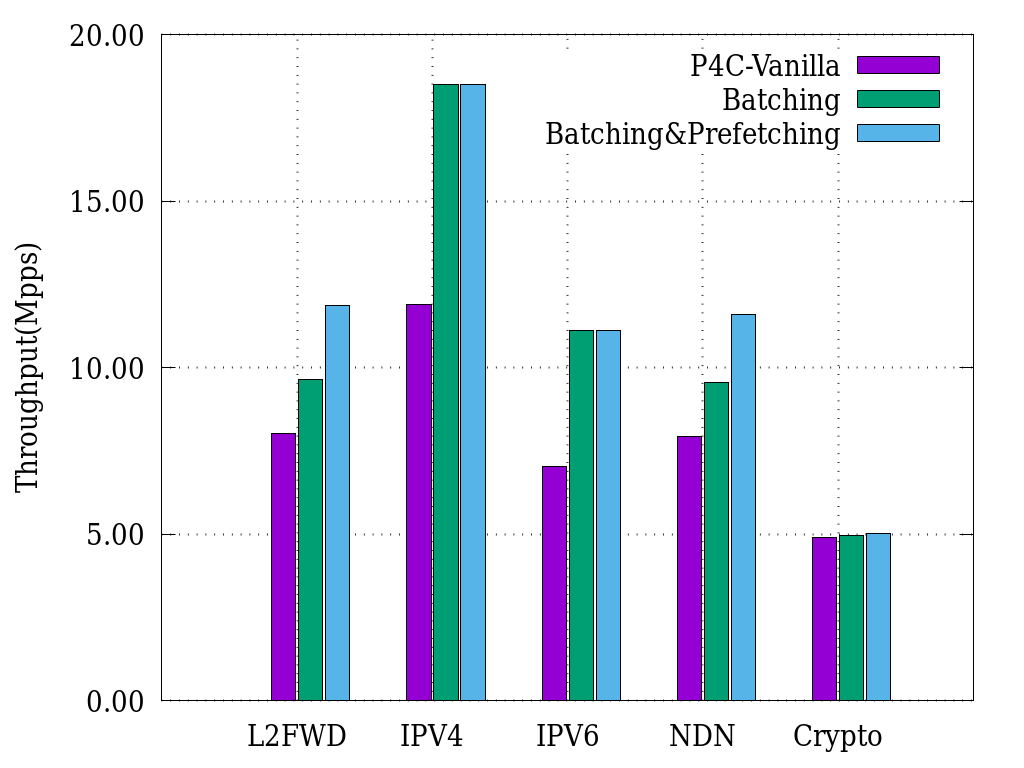
\includegraphics[width = \linewidth]{Figures/effectofbatching.png}
\caption{Effect of batching and prefetching}
\label{batchingandprefetchingfigure}
\end{figure}
In P4C\cite{Laki:2016:HSP:2934872.2959080}, authors are not using batching and prefetching for the applications. We are adding batching and prefetching for all the applications and in Figure \ref{batchingandprefetchingfigure} we are showing the effect of these optimizations for different applications. We are using 32 as batch size for all the applications in all the experiments unless specified otherwise. L2Fwd and NDN are using hash lookup and DPDK code is written in such a way that we are able to prefetch the bucket where the key is present. On the other hand, we don't have much opportunity to use prefetches for LPM lookup based applications. For L2Fwd, batching improves the performance by 20\% and prefetching, used with batching, again improves the performance by 23\%. Similarly for NDN, batching alone improves the performance by 20\% and after adding prefetching there is an additional performance gain of 21 \%. After applying batching and prefetching to IPv4 and IPv6 there is a performance gain of 55\% \& 57\% respectively.
\\
\\
\textbf{Conclusion:} As we can see that batching can be used for almost all the applications without thinking much. The only challenge is to come up with the optimal batch size. Section \ref{optimalbatchsize} can be used to find the optimal batch size. Prefetch on the other hand surely improves the performance but can't be used in every application and should be used with precaution as it might pollute the cache which might result in performance loss.

\subsection{Comparison with hand-tuned applications}
\label{comparisonexperiment}
\begin{figure}[ht]
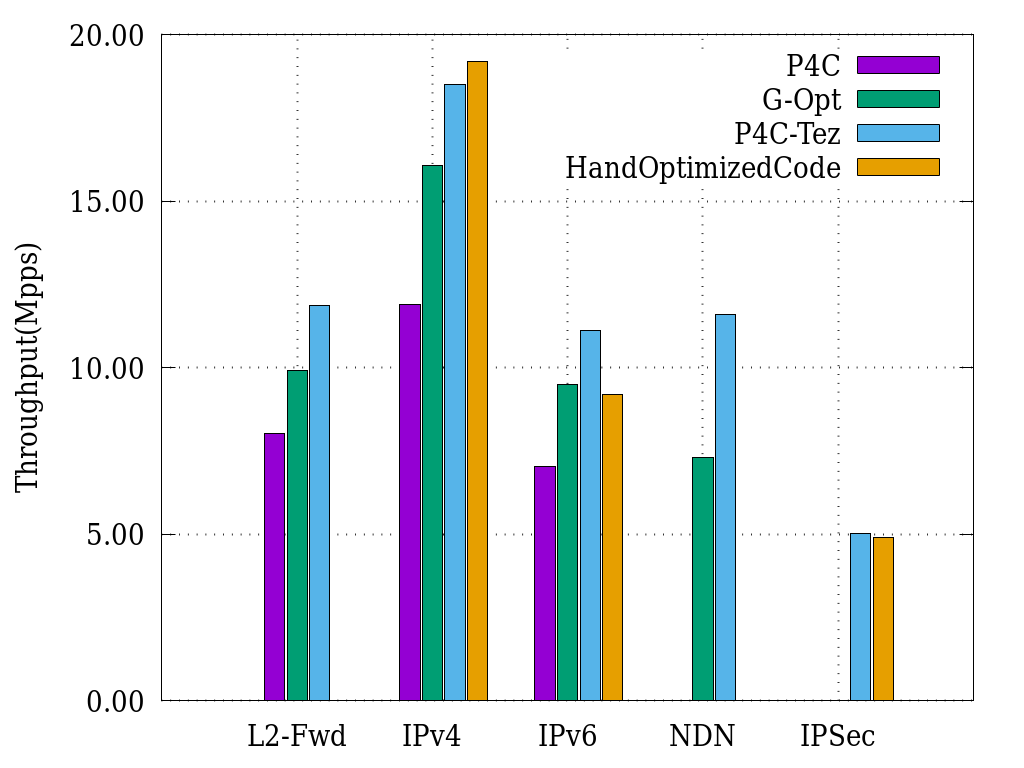
\includegraphics[width = \linewidth]{Figures/comparison.png}
\caption{Comparison with other hand-tuned applications}
\label{comparisonfigure}
\end{figure}
In Figure \ref{comparisonfigure}, we are comparing our automatic generated code with comparable hand-tuned code and vanilla P4C\cite{Laki:2016:HSP:2934872.2959080}. We are making sure that number of lookups and number of entries in the table(s) are same in all the cases so that we can show the comparison among applications. For some of the applications it is not possible to compare our application with the hand-tunes application and we have omitted the bar from the graph for such applications.
\\
\textbf{Comparison with vanilla P4C\cite{Laki:2016:HSP:2934872.2959080}:} This is the most suitable comparison because we are using the same applications and same flow in our applications. There is 48\%, 55\%, 57\%, and 46\% improvement for L2Fwd, IPv4, IPv6, and NDN application respectively. In the applications, they are not exploiting batching \& prefetching and just with these optimizations there is a huge improvement.
\\
\textbf{Comparison with G-Opt\cite{189006}:} There is 20\%, 15\%, 17\%, 59\% improvement for L2Fwd, IPv4, IPv6, and NDN application respectively. They are using both batching and prefetching, and there main aim was to make the results comparable to GPU. The difference is due to the batch size, they are not using the optimal batch size and we can see the performance gain by using the optimal batching size in Figure \ref{tablesize}.
\\
\textbf{Comparison with DPDK\cite{DPDK}:} For IPv4 DPDK is performing 4\% better than our code and for IPv6 we have a performance gain of 20\%. The result for IPv6 doesn't include the improvement we are gaining by TRIE compression, that will be reported later in this section. 
\\
\\
\textbf{Conclusion:} By using the optimal batch size and right prefetch distance we are performing almost equal or better than other hand-tuned optimized code. Even if the results are equal we can say that our approach is better than hand-tuned one, because it is one-time efforts and can be used for wide variety of applications. Results in figure \ref{comparisonfigure} are for one core and we will show in Section \ref{scalability} that our applications are scaling linearly with the number of cores.


\subsection{Scalability}
\label{scalability}
\begin{figure}[ht]
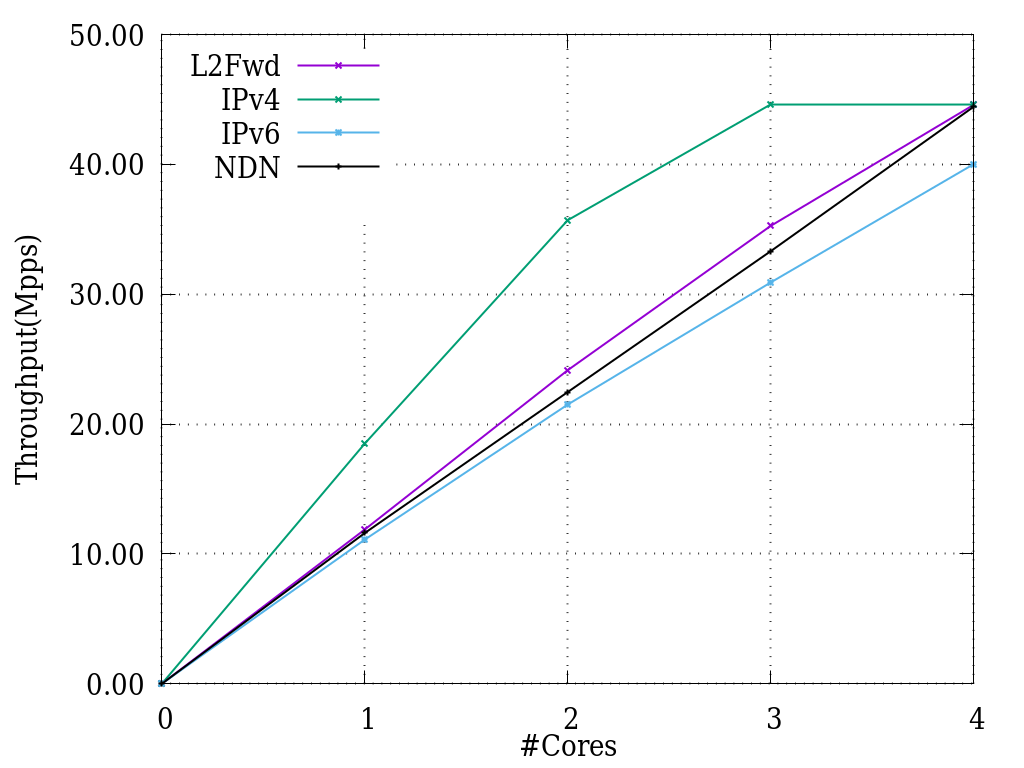
\includegraphics[width = \linewidth]{Figures/cores.png}
\caption{Number of Cores vs Throughput}
\label{cores}
\end{figure}
In Figure \ref{cores}, we are showing that our applications are scaling with the number of cores. With 4 cores we saturating 4 ports(4 x 10 Gbps) when the packet size is 64 bytes.
The theoretical limit for 4 NICs is 59 Mpps but we are getting 44 Mpps as shown in the graph. PCIe is the bottleneck in this case and not the applications. When one NIC is sending and receiving at both the port then it can reach up 22 Mpps and not theoretical maximum 29 Mpps. \cite{Zhou:2013:SHP:2535372.2535379} has also mentioned about this bottleneck in the paper.

There is not much to talk about L2Fwd and NDN application, these applications are scaling linearly. IPv6 is not reaching upto 44 Mpps with 4 cores and that is because of large packet size for IPv6. We are using 64 bytes packets for other applications but Pktgen-DPDK is generating 78 bytes packets for IPv6. Hence IPv6 application is also saturating the ports with 4 cores. The other interesting part of the graph is the IPv4 line, till 2 cores the application is scaling linearly and after that it is coming down. There is no more available bandwidth for the application and it is saturating it with three cores. 
\\
\textbf{Conclusion:}We can say two things about the result of this experiment. First, applications are scaling linearly with the number of cores and second, applications are saturating four 10 Gbps ports with four cores.

\subsection{Relation between Batch Size, Table Size, and Throughput}
\label{batchvstable}
\begin{figure}[ht]
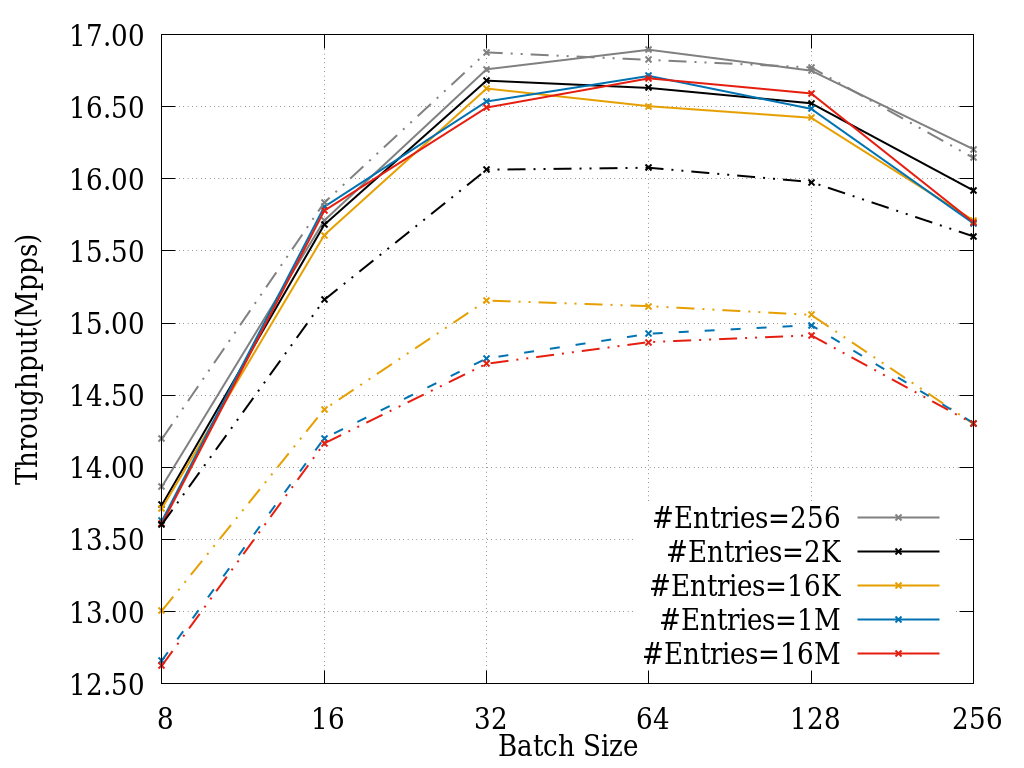
\includegraphics[width = \linewidth]{Figures/TableSizeVsbatchSize.png}
\caption{Throughput vs Batch Size}
\label{tablesize}
\end{figure}
In Figure \ref{tablesize}, we are showing the relation between throughput and batch size for different number of entries in the lookup table. We are using L2-FWD application with one lookup for this experiment. In the graph solid lines are representing the results for batching plus prefetching case and dotted lines are representing batching only results. In case of batching plus prefetching the throughput for same batch size is not varying much when we are varying the entries from 256 to 16 Million, but for same batch the throughput is varying a lot with different number of entries in the table. The throughput is more when the number of entries are less and the throughput is less when the number of entries in the table are more. In Section \ref{batchingsubsection} we will talk about effect of batching on the application with varying number of entries in the table and in Section \ref{prefetchingsubsection} we will take both batching and prefetching into consideration.

\subsubsection{Effect of Batching}
\label{batchingsubsection}
The throughput is decreasing with increase in number of entries for the same batch size. This kind of behavior is expected and can be explained with the help of Eq. \ref{compute_througput}. Eq. \ref{compute_througput} and Eq. \ref{cycles_compute} tell that with the help of batching we can amortize per packet cost and the throughput of the application is improved. There is an improvement in the throughput until we are increasing the batch size from 1 to optimal batch size and after that there is a decline in the throughput. We will explain later in the section why the throughput is decreasing if we are increasing the batch size to more than the optimal batch size.  
\\
\textbf{Batch Size vs Throughput:} In all the cases there is an improvement with the increase in the batch size until the batch size is the optimal batch size for the application and then the application throughput starts decreasing after that. Optimal batch size is different for different cases and can be explained individually for each case. When tables size is small and can fit in L1/L2/L3, the optimal batch size is 32 and if we are increasing the batch size more than 32 then there is a small dip in performance because of the increased cache contention due to increased batch size. However when the table size is bigger than the LLC, for every packet the fetch time is constant and we can increase the batch size to get the benefits of batching. In case of large table size the optimal batch size is 128 in our case.
\\
\textbf{Table Size vs Throughput:} As mentioned in the eq \ref{compute_througput}, memory stall is one of the parameters which is affecting the application throughput. Contention for cache will increase with increase in the number of entries in the lookup table and this will increase the fetch time for lookup data. So, total fetch time will be more for large table size and less for smaller table size. 

As explained in Eq \ref{cycles_stall}, we can hide the memory stalling by prefetching the data in cache. If we can prefetch the data efficiently before the data is used by the application then the total stall time for the batch would decrease and there will be a performance gain.
\subsubsection{Effect of Batching and Prefetching}
\label{prefetchingsubsection}
With prefetching we are trying to minimize the total stall time for the batch and we can see in the figure that there is a performance gain if we are using prefetching with batching. 

\textbf{Table Size vs Throughput:} We can summarize the result in two main points. First, there should be a decline in the throughput with increase in the number of entries and throughput of the application should be more when there are less number of entries in the table. If the memory pressure is more the number of stall cycle will be more and the performance of the application would decrease. For larger table size, data won't be present in the cache and application must stall on it. However, we are prefetching the data even before the data is used in the application and this prefetching of data is reducing the total stall cycles as described in Eq \ref{cycles_stall}. This is the reason that the throughput of the application is stable and not varying much with increase in the number of entries in the table. 

Second, for each batch size the relative throughput of the application will be dictate by the number of entries in the table. In actual, the results are quite opposite to the expectations and this is because total stall time reduction is dependent on effective prefetch distance. One batch size may not work for different number of entries and relation between table size, batch size, and effective prefetch distance has been summarized in Section \ref{subbatching}. Let's take an example of batch size 64, the throughput of the application is more when there are 1 M and 16 M entries as compared to 2 K \& 16 K entries in the table. The data will be in L2/L3 cache for these many number of entries and due to large batch size, entries will be prefetched way before the data will be needed in the application. On the other hand for larger table sizes, larger batch size is suitable since the data will be prefected from the main memory which will take more number of cycles. For 2 K and 16 K entry table we tried to minimized the prefetch distance by using the sub-batch size of 32 and the application is performing better than the application with 1 M and 16 M entries.

\textbf{Conclusion:} 
Application is behaving differently with varying table size, and the optimal batch size is different for different cases. In Section \ref{optimalbatchsize} we have included important factors which can be used to decide the optimal batch size and with this experiment we are making sure that our model is working the way we were expecting.

In case of batching only, the performance is decreasing with an increase in table size because of the increase in the stall time. We are using prefetching to minimize the stall time and in case of batching plus prefetching, the throughput is not declining much due to increase in the table size and we can say that batching and prefetching is playing well together and due to this the throughput is stable even if we are increasing the table size. However 

\subsection{TRIE Compression}
The DIR24-8\cite{Gupta98routinglookups} based Trie IPv6 lookup doesn't exploit the fact that i) many IPv6 prefixes comes from same domain and large portion of their prefixes are common. The DIR24-8 data-structure allocates a 256 entry sized tbl8 even for a single IPV6 entry. This type of over-provisioning leads to memory wastage and also increases memory accesses during lookup. ii) IPv6 prefixes coming from unique domain will be stored in a single node only regardless of its length. Despite having storage overheads compressed trie based lookup outperforms conventional lookup, based on simple trie, by avoiding very costly memory operations involved in accessing a new node. Due to compression there is a dip of 3.5\% in worst case and there is gain of 38\% in best case. Vanilla P4C throughput for IPv6 is 7.2 Mpps and after compression we are getting 8.82 Mpps, which is a performance gain of 22\%. We are getting this performance for the IPv6 entries we are using and we are not checking for best case and worst case performance gain by the compression.

\section{Related Work}
\label{relatedwork}
\textbf{CPU based packet processing:} RouteBricks\cite{dobrescu2009routebricks} is one of the first paper in this area. They exploited various components in a commodity server to achieve 35 Gbps throughput for Layer 3 Forwarding. They used both inter-server and intra-server optimizations to achieve this throughput.
\\
\textbf{Manual optimizations:} There are many papers where authors have come up with different kind of manual optimizations to show the improvement in the performance. Batching\cite{dobrescu2009routebricks, 189006, Kim:2012:PBC:2349896.2349910, Zhou:2013:SHP:2535372.2535379} has been used extensively by authors, however, these papers are determining the batch size by empirical analysis. \cite{189006, Zhou:2013:SHP:2535372.2535379} are exploiting the fact that CPU and Memory subsystem can work in parallel and memory stall can be minimized by issuing the software prefetches before actually using the data. However, it is difficult to use these manual optimizations each time we are writing a packet processing application.
\\
\textbf{Compiler optimizations:} Shangri-La \cite{Chen:2005:SAH:1065010.1065038} generates optimized binary for network processor and showing that the generated binary is working as good as hand-tuned code. \cite{Dobrescu:2010:CPM:1921151.1921154} talks about the importance of doing the optimizations in the compiler rather than hand-tuning the same thing for different applications. The main focus of paper \cite{Dobrescu:2010:CPM:1921151.1921154} is to automating the decision of breaking the application in parallel components to achieve high throughput.
Due to space constraint, we are not mentioning papers related to various kind of software based packet processors and different DSLs for writing the network applications.

\section{Conclusion}
\label{section6} 
The goal of this paper is to find the efficient batch size and right prefetch distance to use the underlying hardware efficiently and to improve the application performance. In the evaluation section, we are showing that per core performance for different applications is on par with hand-tuned optimized applications and applications are scaling with the number of cores. It saves a lot of time and efforts, and we don't need to think about the code flow for different types of applications and the possible bugs due to manual intervention. We believe that DSLs won't be very useful if we are unable to develop good compilers. The actual power of DSLs can only be realized when the compilers can generate the optimized target which is on par with hand-tuned code.

\bibliographystyle{ACM-Reference-Format}
\bibliography{database}
\end{document}
